% PLEASE USE THIS FILE AS A TEMPLATE
% Check file iosart2x.tex for more examples

% add. options: [seceqn,secthm,crcready]
\documentclass[aac,crcready]{iosart2x}

%\usepackage{dcolumn}

%%%%%%%%%%% Put your definitions here


%%%%%%%%%%% End of definitions

\pubyear{0000}
\volume{0}
\firstpage{1}
\lastpage{1}


\begin{document}

\begin{frontmatter}

%\pretitle{}
{\centering \title{Using Tableau as Visualization Tool for MIMIC-III Data
%- Lessons Learned/A (technical) Case Report
}}
\runtitle{Tableau as Tool for Time Series Visualization}
%\subtitle{}

% For one author:
%\author{\inits{N.}\fnms{Name1} \snm{Surname1}\ead[label=e1]{first@somewhere.com}}
%\address{Department first, \orgname{University or Company name},
%Abbreviate US states, \cny{Country}\printead[presep={\\}]{e1}}

% Two or more authors:
\author[A]{\inits{K.}\fnms{Karl} \snm{GOTTFRIED}\ead[label=e1]{k.gottfried@uke.de}%
\thanks{Corresponding Author, Karl Gottfried, Applied Medical Informatics, Hamburg, University Hospital Hamburg-Eppendorf, Martinistraße 52, 20246 Hamburg, Germany;  \printead{e1}.}},
\author[A]{\inits{S.}\fnms{Sylvia} \snm{NÜRNBERG}\ead[label=e2]{second@somewhere.com}}
and
\author[A]{\inits{F.}\fnms{Frank} \snm{ÜCKERT}\ead[label=e3]{third@somewhere.com}}
\address[A]{Applied Medical Informatics, , Germany, \orgname{University Hospital Hamburg-Eppendorf},
\cny{Germany}\printead[presep={\\}]{e1}}
\address[B]{Department first, \orgname{University or Company name},
Abbreviate US states, \cny{Country}\printead[presep={\\}]{e2,e3}}


\begin{abstract}
The meaningful visualization of clinical records can help to facilitate interpretation and exploration among physicians scientists or clinicians, especially with extensive data sets. The MIMIC-III database is an intensive care database, which documents in detail the course and treatment of more than 40,000 patients and can be used as the basis for visualization tools in the medical field. In the present work, we developed exemplary dashboards with Tableau software, that display time series for individual patients and for a selected cohort on the MIMIC-Database. Once created, dashboards can be adapted for specific queries by implementing of dynamic parameters and thus reused. This enables the interactive visualization and exploration of clinical data for non-technical users and also allows them to create customized dashboards.
\end{abstract}

\begin{keyword}
\kwd{Tableau}
\kwd{Data Visualization}
\end{keyword}

\end{frontmatter}

%%%%%%%%%%% The article body starts:

\section{Introduction}\label{s1}

\subsection{Background}\label{s1.1}
\noindent Tableau is a software platform designed for visual exploration and was initially developed and used for data analysis outside of the medical field ~\cite{Ko.2017} [Literatur Tableau seite]. Due to the continuously growing amounts of data and the desire to be able to use this information more efficiently in a clinical and scientific context, the medical field has also become a possible application for data visualization tools such as Tableau ~\cite{Ko.2017} [weitere Literatur]. A clinical data source that has already been used to visualize patient data is the MIMIC-III (Medical Information Mart for Intensive Care) database, a freely accessible critical care database~\cite{Festag.2019,Lee.2016,Johnson.2020,Johnson.2016}. The third version of the MIMIC data set (MIMIC III) contains extensive clinical parameters of more than 40,000 patients who were admitted and treated in medical intensive care units of the Beth Israel Deaconess Medical Center (Boston, Massachusetts, USA) between 2001 and 2012. Data classes ranges from clinical measurements like nurse-verified physiological measurements, laboratory test results or administrative
information like Current Procedural Terminology (CPT) codes and Diagnosis-Related Group (DRG) codes or patient characteristics like Demographic detail and dates of death to free-text interpretations of imaging studies provided by the radiology department ~\cite{Johnson.2020,Johnson.2016}. The data was first deidentified in accordance with Health Insurance Portability and Accountability Act standards before it was incorporated into the database. Furthermore to protect the privacy of the patients, researcher have to pass an online course and accept a data use agreement before they get access to the database ~\cite{Johnson.2020,Johnson.2016}. A demo data set with 100 patients is provided without restriction for test purposes.


\subsection{Objective and Requirements}\label{s1.2}
The objective of this work is to provide a template for a visual data analysis and exploration tool for time series values, so that medically trained researchers can obtain clinical information more easily.
The requirements to be met by the implemented dashboards are:
\begin{itemize}
\item A user can display the course of time-dependent variables like blood pressure over time for a patient or for a cohort and dynamically adjust the variable.
\item The user can select a patient cohort by dynamic filtering of variables contained in the data.
\item The dashboards should be easily expandable so that, medically trained researchers can make their own basic extensions or additions to the dashboards.
\end{itemize}

\section{State of the art}\label{s2}



\section{Concept}\label{s3}
For our implementation we used the commercially available software Tableau Desktop provided by Tableau\textregistered. The interaction with Tableau Desktop works by translating drag-and-drop actions into data queries via an intuitive user interface. For a first introduction of the user interface see also Ko and Chang~\cite{Ko.2017}. 
Tableau can be connected to multiple data sources like spreadsheets or text files, or for instance in a big data, relational database on a server. Here we used the provided 26 comma-separated values (CSV) files and build the corresponding data model based on the information about the MIMIC-III data structure provided by the PhysioNet website (https://mimic.physionet.org/). Fig.~\ref{f1} shows an overview over the used data model to interact with the data. So-called worksheets are used as the basis for creating dashboards and can be individualized depending on the question. For the visual representation of the existing data, Tableau uses a total of four possible forms of the data values. Tableau uses the following measurement types: a) continuous aggregate measure, b) discrete aggregate measure, c) continuous disaggregate measure, d) discrete disaggregate measure in which b) and d) are considered as dimensions by Tableau.
New data values can be added via so-called calculated fields and also displayed in the visualization. Tableau uses its own calculation syntax for the calculated fields that is reminiscent of Excel statements. Using so-called filters, data rows can be selected and also be changed dynamically using parameters. With these tools, worksheets can be specially adapted and thus used as a basis for dashboards. Dashboards are another way of interaction for the user, as individual worksheets can be linked using so-called actions.

\begin{figure}[t]
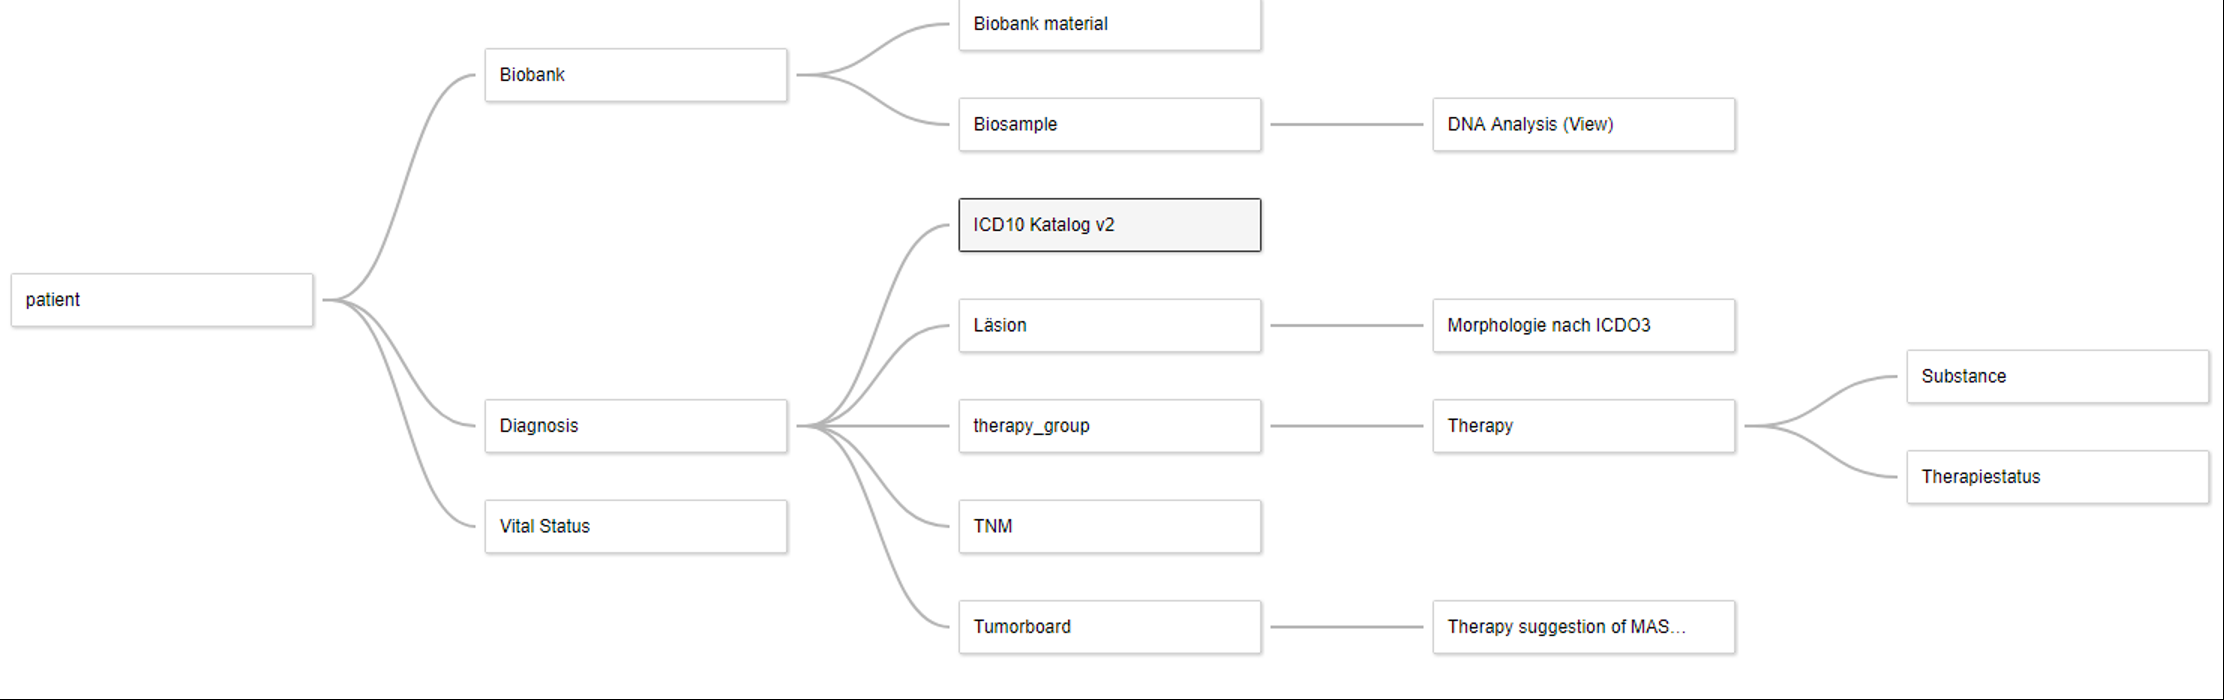
\includegraphics[width=0.7\textwidth]{images/datamodel_1.png}
\caption{Representation of the MIMIC Data Model: The squares represent CSV data tables the connections between the data tables represent the join relations used}\label{f1}
\end{figure}

\section{Implementation}\label{s4}



\section{Discussion and Outlook}\label{s5}
The dashboards created with Tableau Desktop represent a customizable and expandable presentation of clinical data. It is easy to imagine that, in addition to the area of application shown, other recurring questions can be presented, such as ...
A major limitation regarding the reusability of worksheets and dashboards with Tableau is that the visualizations or calculations depend on the correct designation and the data type used. If the name or type of a data field changes in the underlying data model over time, it may be that all the visualizations and calculations that are dependent on it have to be adapted accordingly and cannot be used. Reusability could be increased through a uniform and generally applicable data model. It is conceivable, for example, that the visualization shown is based on a general data model such as SNOMED CT instead of the MIMIC data model and can act as the basis for the data model.

\section{Conclusion}\label{s6}
Using Tableau Software, we developed two interactive dashboards to display time-dependent variables. The approach presented can be expanded or adapted depending on the context and thus supplement already established analysis methods for specific questions. An implementation of the presented dashboard is available at ...



%\begin{figure}[t]
%\includegraphics{}
%\caption{Figure caption.}\label{f1}
%\end{figure}

%\begin{table*}
%\caption{} \label{t1}
%\begin{tabular}{lll}
%\hline
%&&\\
%&&\\
%\hline
%\end{tabular}
%\end{table*}

%%%%%%%%%%% The bibliography starts:

%%%%%%%%%%%%%%%%%%%%%%%%%%%%%%%%%%%%%%%%%%%%%%%%%%%%%%%%%%%%%
%%                  The Bibliography                       %%
%%                                                         %%
%%  ios1.bst will be used to                               %%
%%  create a .BBL file for submission.                     %%
%%                                                         %%
%%                                                         %%
%%  Note that the displayed Bibliography will not          %%
%%  necessarily be rendered by Latex exactly as specified  %%
%%  in the online Instructions for Authors.                %%
%%                                                         %%
%%%%%%%%%%%%%%%%%%%%%%%%%%%%%%%%%%%%%%%%%%%%%%%%%%%%%%%%%%%%%


\nocite{*} 
% if your bibliography is in bibtex format, use those commands:
\bibliographystyle{ios1}           % Style BST file.
\bibliography{bibliograpy_tableau.bib}        % Bibliography file (usually '*.bib')

% or include bibliography directly:
%\begin{thebibliography}{0}
%\bibitem{r1} F. Author, Information about cited object.
%
%\bibitem{r2} S. Author and T. Author, Information about cited object.
%\end{thebibliography}

\end{document}
